
\documentclass[border=4pt]{standalone}
\usepackage{amsmath,amssymb}
\usepackage{tikz}
\usetikzlibrary{arrows.meta,positioning,shapes.geometric,calc,shadows}
\usepackage[scaled=0.92]{helvet}
\tikzset{
  box/.style={draw, rounded corners, fill=white, minimum width=0.85cm, minimum height=0.55cm, inner sep=2pt},
  st/.style={fill=gray!30, draw, regular polygon, regular polygon sides=3, inner sep=0pt, minimum size=4mm},
  ef/.style={fill=gray!30, draw, regular polygon, regular polygon sides=3, shape border rotate=180, inner sep=0pt, minimum size=4mm},
  cp/.style={circle, fill, inner sep=1.3pt},
  wl/.style={inner sep=1.5pt, font=\small},
  v/.style={circle, draw, inner sep=1pt, minimum size=7.5mm, font=\normalsize},
  hv/.style={circle, draw, dashed, inner sep=1pt, minimum size=7.5mm, font=\normalsize, fill=gray!10},
  >=Stealth, line width=0.5pt
}
\begin{document}

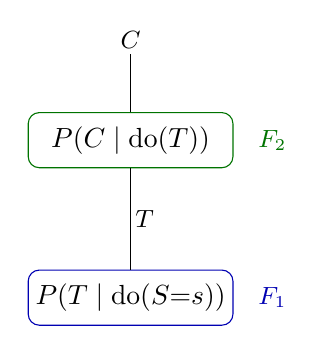
\begin{tikzpicture}
\node[box, minimum width=2.6cm, minimum height=0.7cm, draw=blue!70!black] (b1) at (1.6,1.0) {$P(T \mid \mathrm{do}(S{=}s))$};
\node[box, minimum width=2.6cm, minimum height=0.7cm, draw=green!45!black] (b2) at (1.6,3.0) {$P(C \mid \mathrm{do}(T))$};
\draw (b1.north) -- (b2.south) node[midway, right, wl]{$T$};
\draw (b2.north) -- (1.6,4.1) node[wl,above]{$C$};
\node[blue!70!black, font=\small, anchor=west] at (3.1,1.0) {$F_1$};
\node[green!45!black, font=\small, anchor=west] at (3.1,3.0) {$F_2$};
\end{tikzpicture}
\end{document}